\subsection{A Two-Phase Query Answering Framework}
The formulation above highlights that counterfactual retrieval is not a simple extension of nearest-neighbor search. A counterfactual engine must enforce instance-level semantics $\omega$, which define feasibility and transformation cost, and return a size-$k$ \emph{set} whose overall utility is determined by a set-level objective $\Omega$.

\begin{figure*}[t]
\centering
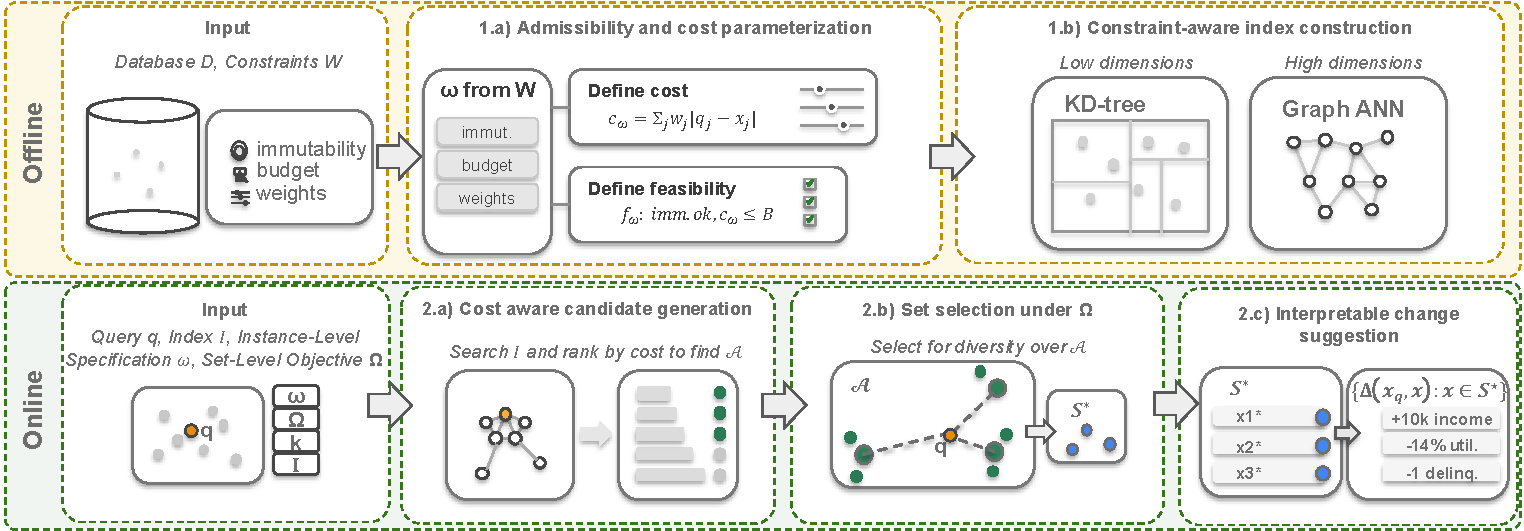
\includegraphics[width=0.84\textwidth]{figs/cfvision_graphics_editable_v10.pdf}
\caption{Two-phase counterfactual query pipeline.} 
\label{fig:cf_two_stage_pipeline}
\end{figure*}

%\subsection{Two-Phase Execution System}

To realize our vision in system design, we develop a two-phase framework for answering counterfactual queries. Unlike nearest-neighbor search, counterfactual querying must enforce instance-level semantics $\omega$ (feasibility and cost) and optimize a set-level objective $\Omega$. This requires tightly integrating constraint-aware retrieval with set-level optimization.

The framework consists of an offline phase that prepares reusable structures over $\mathcal D$ and a specification space $\mathcal W$, and an online phase that answers queries $(q,\omega,\Omega,k)$ efficiently using these structures.

\subsubsection{Offline (Preprocessing for $(\mathcal D,\mathcal W)$)}
Given $\mathcal D$ and a \emph{specification family} $\mathcal W$, \rev{i.e., a set of specifications $\omega$ that share the same structural primitives---the same immutable attributes, constraint types, and cost components---and therefore admit a common index, differing only in their concrete parameters (e.g., per-attribute weights or thresholds),} the system builds reusable components to support efficient evaluation of feasibility and cost under different $\omega \in \mathcal W$. First (\textbf{Step 1.a}), it identifies structural primitives that define admissibility and transformation cost, such as immutable attributes, constraint types, and cost components. These primitives parameterize $\omega$ at query time. Second (\textbf{Step 1.b}), it constructs a constraint-aware index $\mathcal I$ over $\mathcal D$, organized according to the structure induced by $\mathcal W$, so that queries can be efficiently evaluated under different specifications.

The design of $\mathcal I$ depends on the role of $\omega$. For example, when $\omega$ mainly reweights dimensions, metric-aware structures (e.g., weighted KD-trees~\cite{reif2022scalable}, ball trees~\cite{dolatshah2015ball}, cover trees~\cite{izbicki2015faster}) enable efficient pruning. When $\omega$ is dominated by discrete constraints, techniques such as partitioned indices~\cite{lee2019constraint}, bitmap filtering~\cite{chan1998bitmap}, or inverted indices~\cite{babenko2014inverted} can filter infeasible candidates before cost evaluation.

\paragraph{Online (querying over $(q,\omega,\Omega,k)$).}
Given a query $(q,\omega,\Omega,k)$, directly optimizing Eq.~\eqref{eqn:objective} is computationally expensive. We can therefore adopt a coarse-to-fine strategy that leverages $\mathcal I$.

First (\textbf{Step 2.a}), it retrieves a candidate pool $\mathcal A_\omega(q)$ consisting of admissible instances $\mathbf{x}$ with low cost $\omega(\mathbf{x}_q,\mathbf{x})$, returned in nondecreasing cost order for early pruning. Note that, if $\omega \notin \mathcal W$, the system falls back to a linear scan over $\mathcal D$. Formally,
\begingroup\small
\begin{equation}
\mathcal A_\omega(q) 
\in 
\arg\min_{\substack{\mathcal A_\omega \subseteq \mathcal \omega(q)\\ |\mathcal A_\omega|=m}}\left\{
\sum_{\mathbf{x}\in \mathcal A_\omega} \omega(\mathbf{x}_q,\mathbf{x})\right\},
\end{equation}
\endgroup
where $m \ge k$ controls the pool size.

Second (\textbf{Step 2.b}), it selects the final set $S^\star \subseteq \mathcal A_\omega(q)$ by optimizing Eq.~\eqref{eqn:objective}, balancing transformation cost with the set-level objective $\Omega$ (e.g., diversity, robustness, fairness). Finally (\textbf{Step 2.c}), for each $\mathbf{x} \in S^\star$, the system produces an interpretable edit $\Delta(\mathbf{x}_q, \mathbf{x})$ that specifies how to transform $\mathbf{x}_q$ into $\mathbf{x}$, consistent with $\omega$.

\rev{This coarse-to-fine design bounds the cost of constraint enforcement and feasibility validation. Cheap attribute- and metric-level checks are performed during candidate generation (Step~2.a), pruning most infeasible instances before any expensive validation. Costly execution-level (temporal, graph) or semantic (text, image) validation is then applied only to the small candidate pool $\mathcal A_\omega(q)$, so validation cost scales with $|\mathcal A_\omega|$ rather than $|\mathcal D|$. Since candidates are returned in nondecreasing cost order, validation terminates once $k$ admissible answers are found. Increasing the pool size $m$ improves the likelihood of finding $k$ feasible counterfactuals at the expense of additional validation, providing a controllable accuracy--latency trade-off (Principle P3 in Section~\ref{sec:core_principles}).}

%Figure~\ref{fig:cf_two_stage_pipeline} illustrates the overall framework for counterfactual queries. In the offline stage, the system first performs \emph{1.a) Admissibility and cost parameterization} by examining the parameter space and selecting a configuration $\omega \in \mathcal{W}$, which defines the admissibility rules and transformation cost, where infeasible changes are assigned infinite cost. It then performs \emph{1.b) Constraint-aware index construction}, building a reusable index $\mathcal{I}$ over $\mathcal{D}$ to support efficient retrieval under these instance-level semantics. The index design is determined by the geometry induced by $\omega$. When $\omega$ restricts changes to a small mutable subspace or emphasizes a limited number of weighted dimensions, tree-based indices are typically effective. When $\omega$ allows greater flexibility or operates over high-dimensional representations, graph-based approximate nearest neighbor indices are more suitable.

%In the online stage, given the prebuilt index $\mathcal{I}$, the system proceeds in three steps. First, \emph{2.a) Cost-aware candidate generation} retrieves and ranks admissible instances under $\omega$, producing a candidate pool $\mathcal{A}_\omega(q)$ (green nodes) for query $q$ (orange node). Next, \emph{2.b) Set selection under $\Omega$} selects the final response set $S^\star \subseteq \mathcal{A}_\omega(q)$ (blue nodes) to optimize the specified set-level objective. Finally, \emph{2.c) Interpretable change selection} returns $S^\star$ together with domain-level edit descriptions $\Delta(q,x)$ for each selected instance $x \in S^\star$.
\subsection{Core Principles}\label{sec:core_principles}

The formulation above exposes the key requirements for counterfactual querying: results must be actionable, cost-faithful, scalable, and informative as a set, which can be distilled into four core principles for system design.

\paragraph{\textbf{P1 (Interpretability).}} 
\emph{Counterfactual results must be interpretable in the original domain}. For each selected counterfactual $\mathbf{x} \in S^\star$, the system returns a domain-level edit $\Delta(\mathbf{x}_q,\mathbf{x})$ (e.g., feature changes in tabular data or valid edit sequences in structured data). Both the representation and index must preserve sufficient information to reconstruct $\Delta(\mathbf{x}_q,\mathbf{x})$, and the cost $\omega(\mathbf{x}_q,\mathbf{x})$ must be grounded in this edit. Thus, the result is tied to actionable transformations rather than similarity, supporting human-centered reasoning.

\paragraph{\textbf{P2 (Cost faithfulness).}} 
\emph{The cost function $\omega(\mathbf{x}_q,\mathbf{x})$ must reflect true intervention effort}. If $\omega(\mathbf{x}_q,\mathbf{x}_a) < \omega(\mathbf{x}_q,\mathbf{x}_b)$, then transforming $\mathbf{x}_q$ to $\mathbf{x}_a$ should be no harder than to $\mathbf{x}_b$ under the intended domain model. Infeasible transformations are assigned infinite cost, cleanly separating feasibility from effort. This principle anchors retrieval in realistic actions, ensuring semantic correctness.

\paragraph{\textbf{P3 (Efficiency).}} 
\emph{The system must efficiently retrieve admissible candidates in $\mathcal \omega(q)$ at scale}. It should provide predictable performance, bounded resource usage, and controllable trade-offs between accuracy and latency. This principle makes the vision practical, enabling deployment over large and heterogeneous datasets.

\paragraph{\textbf{P4 (Collective validity).}} 
\emph{The returned answer set must jointly optimize set-level objectives and transformation cost}. Given $(q,\omega,\Omega,k)$, the solution $S^\star$ satisfies $|S^\star|=k$ and optimizes Eq.~\eqref{eqn:objective}. Since $\Omega$ captures collective criteria such as diversity, robustness, and fairness, the system must balance these objectives against per-instance cost. This elevates query answering from ranking individual instances to constructing informative and complementary sets.

Together, P1--P4 define counterfactual querying as structured, constraint-aware, and set-oriented retrieval rather than similarity search, ensuring actionability, scalability, and collective validity.
\subsection{An Illustrative Example on Tabular Data}

We illustrate how counterfactual querying realizes our vision using a loan approval scenario. Suppose Maya applies for a loan and her application is denied. Her record is
$
\texttt{(Income=\$58k, Util.=41\%, Delinq.=1, State=NC, Age=28)}.
$
She asks: \emph{``What would I need to change to get approved?''} This question is naturally expressed as a counterfactual query $(q,\omega,\Omega,k)$, where $\omega$ encodes feasibility and cost (e.g., age is immutable, effort varies by attribute), $k$ specifies the number of options, and $\Omega$ promotes diverse recourse strategies.

\textbf{Offline.} The system prepares $\mathcal D$ under $\omega$ by defining admissibility and cost (e.g., $\text{Age} \neq 28$ is infeasible) and building a label-aware index $\mathcal I$ over approved records. This ensures traceable edits and cost-faithful ranking (P1--P2), while enabling efficient retrieval (P3).

\textbf{Online.} Given $(q,\omega,\Omega,k)$, the system retrieves a candidate pool of feasible instances with low cost, then selects $k$ answers by optimizing Eq.~\eqref{eqn:objective} to balance effort and diversity (P4). It returns each instance with an interpretable edit $\Delta(\mathbf{x}_q,\mathbf{x})$.

In the end, Maya may receive three complementary paths to approval, such as (i) \texttt{+10k income with -2\% utilization}, (ii) \texttt{-14\% utilization}, or (iii) \texttt{-1 delinquency with -6\% utilization}. These results are grounded in real data (P1), feasible under $\omega$ (P2), efficiently retrieved (P3), and collectively valid under $\Omega$ (P4), illustrating actionable data-centric reasoning.



